\documentclass[leqno]{beamer}
\usetheme{CambridgeUS}    %  other good options:   Singapore, Warsaw, Plain, CambridgeUS, Berlin

%\mode<presentation> {
 % \setbeamertemplate{background canvas}[vertical shading][bottom=white!10,top=white!10]
 %\setbeamertemplate{navigation symbols}{}
 
  %\usefonttheme[onlysmall, nonav]{structurebold}
%}
\usepackage{graphics,multicol,url}
\usepackage{colortbl}
% \usepackage{biblatex}
% \bibliography{JetBib.bib}
\usepackage{amsfonts, amsmath, amssymb, eucal, enumerate,calc,latexsym,amsfonts}
\usepackage{amsmath,amsthm, amssymb, latexsym}
\usepackage{enumerate}
\usepackage{tikz}
\usetikzlibrary{shadings}
\usepackage{gensymb}

\usepackage{amssymb, amsthm, amsmath, amsfonts}
\usepackage{cancel, enumerate, url, mathrsfs}
% \input{dvipsnam.def}
% \usepackage{graphicx}
% \DeclareGraphicsRule{.tif}{png}{.png}{`convert #1 `dirname #1`/`basename #1 .tif`.png}
% \graphicspath{{./figures/}}
 \setbeamertemplate{navigation symbols}{}    % removes the panel with navigation symbols from the lower right corner
% Shows "invisible text"
%\setbeamercovered{still covered={\opaqueness<1->{5}}}

%\setbeameroption{show notes}
%\setbeameroption{show notes on side=left}


\newtheorem{thm}{Theorem}
\newtheorem{cor}[thm]{Corollary}
\newtheorem{lem}[thm]{Lemma}
\newtheorem{prop}[thm]{Proposition}
\theoremstyle{definition}
\newtheorem{defn}[thm]{Definition}
\theoremstyle{remark}
\newtheorem{rem}[thm]{Remark}
%\numberwithin{equation}{section}



\newcommand{\vp}{\varphi}
\newcommand{\re}{\mathbb{R}}
\newcommand{\na}{\mathbb N}
\newcommand{\ra}{\mathbb Q}
\newcommand{\bfx}{\bf x}
\newcommand{\ds}{\displaystyle}
\newcommand{\dint}{\displaystyle\int}
\newcommand{\al}{\alpha}
\definecolor{DarkBlue}{rgb}{0.1,0.1,0.5}
\definecolor{Red}{rgb}{0.9,0.0,0.1}
\newcommand{\brown}[1]{{\color{brown} #1}}
\newcommand{\red}[1]{{\color{red} #1}}
\newcommand{\blue}[1]{{\color{blue} #1}}


\title[Math 107-Lecture 7]{Calculus I - Lecture 7\\Wednesday, September 6, 2017}
\author[A. Larios]{Dr. Adam Larios}
\institute[UNL]{University of Nebraska-Lincoln}
\date{September 6, 2017}

\begin{document}

\frame{\titlepage}
%%%%%%%%%%%%%%%%%%%%%%%%%%%%%%%%%%%%%%%%%%%%%%%%%%%%%%%%%%%


\begin{frame}
\frametitle{Announcements}

\begin{itemize}
\item Today: the derivative function and interpretation of derivative (sections 2.3 and 2.4).
\end{itemize}
\end{frame}



%%%%%%%%%%%%%%%%%%%%%%%%%%%%%%%%%%%%%%%%%%%%%%%%%%%%%%%%%%%


\frame{\frametitle{Computing the Derivative Algebraically}

Find the derivative of $f(x)=1/x$ at the point $x=2$

{\color{blue} Solution:}
The derivative is the limit of the difference quotient, so we look at

\begin{align*}
f'(2)&=\lim\limits_{h \rightarrow 0}\frac{f(2+h)-f(2)}{h} =\lim\limits_{h \rightarrow 0}\frac{\frac{1}{2+h}-\frac{1}{2}}{h}\\
&=\lim\limits_{h \rightarrow 0} \frac{2-(2+h)}{2h(2+h)}=\lim\limits_{h \rightarrow 0}\frac{-h}{2h(2+h)}
\end{align*}
Since the limit only examines values of $h$ close to, but not equal to, zero, we can cancel $h$. We get

\[f'(2)=\lim\limits_{h \rightarrow 0} \frac{-h}{2h(2+h)}=\frac{-1}{4}\]

Thus, $f'(2) = -\ds\frac{1}{4}$. 

}


%%%%%%%%%%%%%%%%%%%%%%%%%%%%%%%%%%%%%%%%%%%%%%%%%%%%%%%%%%%

\frame{\frametitle{Example of a nondifferentiable function}

Let $f(x)=|x+1|$.  Then $f(x)$ is NOT differentiable at $x=-1$.

{\color{blue}Hint:}  Use the limit definition for the piecewise defined function
\[
|x+1|:= \begin{cases}
x+1, \quad x\geq -1\\
-(x+1), \quad x<-1. 
\end{cases}
\]
}


%%%%%%%%%%%%%%%%%%%%%%%%%%%%%%%%%%%%%%%%%%%%%%%%%%%%%%%%%%%
\frame{\frametitle{Tangent lines to the graph of a function}
{\color{blue}Example.} Find the eqn. for the tangent line to $f(x)=x^3+2x$ at $x=-1$. 
\pause

{\color{blue}Solution.} To determine the equation of the tangent line we need:\pause

\begin{enumerate}
\item[(i)] {\color{red}Slope.} The slope of the graph at a point is the same as the slope of the tangent line at that point, which is the value of the derivative.
\begin{align*}
f'(-1)&=\lim_{h\to 0} \frac{f(-1+h)-f(-1)}{h}\\
&=\lim_{h\to 0}\frac{(-1+h)^3 +2(-1+h)-(-1)^3-2(-1)}{h}\\
&=\lim_{h\to 0}\frac{h^3-3h^2+5h}{h}={\color{red}5}
\end{align*}
\vspace*{-.2in}
\pause
\item [(ii)] {\color{green}Point.} The tangent line is at $x=-1$, so we need to find the coordinates of 
$
(-1, f(-1)) = (-1, (-1)^3+2(-1))={\color{green}(-1, -3)}.$
\pause
The eqn. of the tangent line is \fbox{$y-{\color{green}(-3)}={\color{red}5}(x-{\color{green}(-1))}$} or \fbox{$y=5x+2.$}
\end{enumerate} 
}


\frame{\frametitle{Geometric viewpoint}

\begin{multicols}{2}
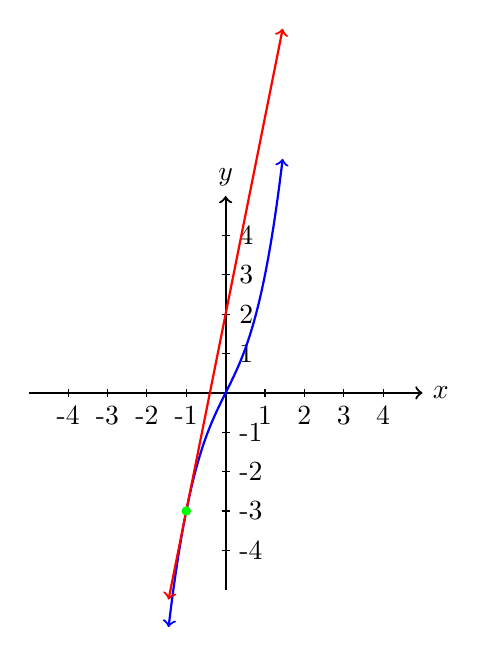
\begin{tikzpicture}[scale=0.5]

    \draw[->,thick] (-5,0) -- (5,0) node[right] {$x$};
    \draw[->,thick] (0,-5) -- (0,5) node[above] {$y$};
	\foreach \x in {-4,-3,-2,-1,1,2,3,4} \draw (\x,0.1) -- (\x, -0.1) node[below] {\x};
	\foreach \y in {-4,-3,-2,-1,1,2,3,4} \draw (-0.1,\y) -- (0.1,\y) node[right] {\y};

\draw[<->,color=black,smooth,domain=-1.45:1.45,thick,color=blue] plot(\x,{\x*(\x)*(\x)+2*(\x)});
\draw[<->,color=black,smooth,domain=-1.45:1.45,thick,color=red] plot(\x,{5*(\x)+2});
\draw[color=green] (-1,-3) circle[radius=3pt];
\fill[color=green] (-1,-3) circle[radius=3pt];

\end{tikzpicture}


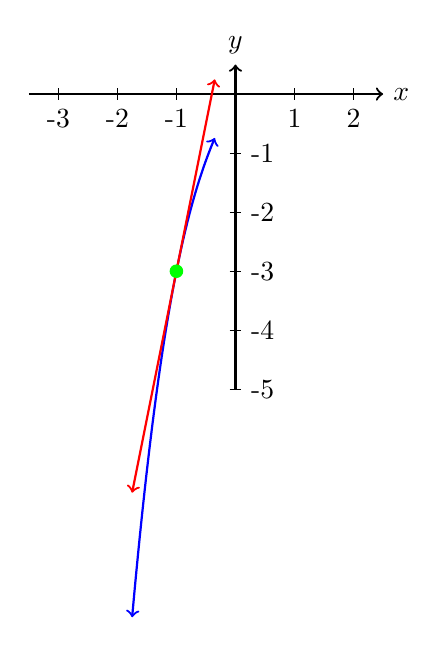
\begin{tikzpicture}[scale=0.75]

    \draw[->,thick] (-3.5,0) -- (2.5,0) node[right] {$x$};
    \draw[->,thick] (0,-5) -- (0,.5) node[above] {$y$};
	\foreach \x in {-3,-2,-1,1,2} \draw (\x,0.1) -- (\x, -0.1) node[below] {\x};
	\foreach \y in {-5,-4,-3,-2,-1} \draw (-0.1,\y) -- (0.1,\y) node[right] {\y};

\draw[<->,color=black,smooth,domain=-1.75:-0.35,thick,color=blue] plot(\x,{\x*(\x)*(\x)+2*(\x)});
\draw[<->,color=black,smooth,domain=-1.75:-0.35,thick,color=red] plot(\x,{5*(\x)+2});
\draw[color=green] (-1,-3) circle[radius=3pt];
\fill[color=green] (-1,-3) circle[radius=3pt];

\end{tikzpicture}

\end{multicols}

}



%%%%%%%%%%%%%%%%%%%%%%%%%%%%%%%%%%%%%%%%%%%%%%%%%%%%%%%%%%%

\frame{\frametitle{Using the derivative for approximations}
We have that the line {\color{red}$y=5x+2$} is tangent to {\color{blue}$f(x)=x^3+2x$} at {\color{green}$x=-1$}. Therefore 
\[
{\color{blue}x^3+2x} \approx {\color{red}5x+2} \quad \text{ for $x$ close to }  {\color{green}-1}.
\] 
Thus
\[
{\color{blue}f(-1.01)=(-1.01)^3+2(-1.01)= -3.050301} \approx {\color{red}\underbrace{5(-1.01)+2}_{=y(-1.01)}=-3.05}.
\]

}


%%%%%%%%%%%%%%%%%%%%%%%%%%%%%%%%%%%%%%%%%%%%%%%%%%%%%%%%%%%

\frame{\frametitle{Clicker question \#1}
What is the slope of the graph of $f(x)=5x^2-2x$ at $x=-2$?
\begin{enumerate}[(A)]
\item 20
\item $-20$
\item $-10$
\item $10$
\item it does not exist
\end{enumerate}
}


%%%%%%%%%%%%%%%%%%%%%%%%%%%%%%%%%%%%%%%%%%%%%%%%%%%%%%%%%%%

\frame{\frametitle{Derivative as a function}
The derivative {\color{blue}function} is defined for every $x$ as the function
\[
f'(x)=\lim_{h\to 0}\frac{f(x+h)-f(x)}{h}
\]
provided the limit exists. Here, we do not specify the point, it is a general $x$.

{\color{blue}Example.} Find $f'(x)$ for $f(x)=2x^2+3x.$

\begin{align*}
f'(x)&=\lim_{h\to 0}\frac{f(x+h)-f(x)}{h}\\
&=\lim_{h\to 0}\frac{2(x+h)^2+3(x+h)-2x^2-3x}{h}\\
&=\lim_{h\to 0}\frac{2x^2+4xh+2h^2+3x+3h-2x^2-3x}{h}\\
&=\lim_{h\to 0}(4x+2h+3)=4x+3.
\end{align*}
}

%%%%%%%%%%%%%%%%%%%%%%%%%%%%%%%%%%%%%%%%%%%%%%%%%%%%%%%%%%%

\frame{\frametitle{Graphically}
Based on the fact that 
\begin{center}
{\color{blue}the slope of the graph=value of derivative} 
\end{center}
we see that
\begin{itemize}
\item If $f'(x)>0$ on an open interval $I$ then $f(x)$ is increasing on $I$.
\item If $f'(x)<0$ on an open interval $I$ then $f(x)$ is decreasing on $I$.
\end{itemize}  
\pause
In the example above, for $f(x)=2x^2+3x$ and $f'(x)=4x+3$ we have
\begin{itemize}
\item $f$ is increasing when $f'(x)=4x+3>0$, i.e. $x\in (-\ds\frac{3}{4},\infty)$
\item $f$ is decreasing when $f'(x)=4x+3<0$, i.e. $x\in (-\infty, -\ds\frac{3}{4}).$
\end{itemize}
}



%%%%%%%%%%%%%%%%%%%%%%%%%%%%%%%%%%%%%%%%%%%%%%%%%%%%%%%%%%%

\frame{\frametitle{Clicker question \#2}
What is the largest set on which the function graphed below is increasing?
\begin{multicols}{2}
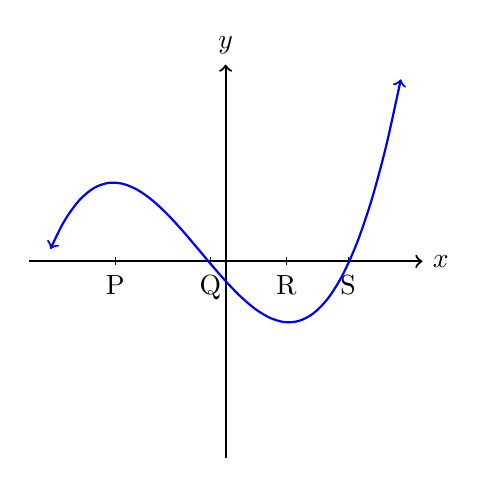
\begin{tikzpicture}[scale=0.5]

    \draw[->,thick] (-5,0) -- (5,0) node[right] {$x$};
    \draw[->,thick] (0,-5) -- (0,5) node[above] {$y$};
	%\foreach \x in {-4,-3,-2,-1,1,2,3,4} \draw (\x,0.1) -- (\x, -0.1) node[below] {\x};
	%\foreach \y in {-4,-3,-2,-1,1,2,3,4} \draw (-0.1,\y) -- (0.1,\y) node[right] {\y};
\draw (-2.8,0.1) -- (-2.8, -0.1) node[below] {P};
\draw (-0.39,0.1) -- (-0.39, -0.1) node[below] {Q};
\draw (1.54,0.1) -- (1.54, -0.1) node[below] {R};
\draw (3.11,0.1) -- (3.11, -0.1) node[below] {S};
\draw[<->,color=blue,smooth,domain=-4.45:4.45,thick] plot(\x,{\x*(\x)*(\x)*0.08+(\x)*(\x)*0.15-1.1*\x-0.5});
\end{tikzpicture}



\begin{enumerate}[(A)]
\item $(-\infty, P)\cup (S,\infty)$
\item $(-\infty, Q)\cup (S,\infty)$
\item $(R, \infty)$
\item $ (-\infty, P)\cup (S,\infty)$
\item $(-\infty, P) \cup (R,\infty)$
\end{enumerate}
\end{multicols}
}

%%%%%%%%%%%%%%%%%%%%%%%%%%%%%%%%%%%%%%%%%%%%%%%%%%%%%%%%%%%

\frame{\frametitle{A few differentiation formulas}

Using the definition of the derivative function we obtain:
\begin{itemize}
\item If $f(x)=k$ with $k$ constant, then $f'(x)=0$.
\item If $f(x)=a+bx,$ with $a,b$ constant, then $f'(x)=b$
\item (Power Rule:) If $n\neq 0$ and $f(x)=x^n,$ then $f'(x)=nx^{n-1}$.
\end{itemize}

\pause
Thus, if $f(x)=\ds\frac{1}{x^{2/3}}=x^{-2/3}$ then $f'(x)=-\ds\frac{2}{3}x^{-\frac{2}{3}-1}=-\ds\frac{2}{3}x^{-\frac{5}{3}}.$ 
}

%%%%%%%%%%%%%%%%%%%%%%%%%%%%%%%%%%%%%%%%%%%%%%%%%%%%%%%%%%%

\frame{\frametitle{Notation}
If $y=f(x)$, then
\[
f'(x)=y'=\frac{dy}{dx}=\frac{df}{dx}=\frac{d}{dx}[y]=\frac{d}{dx}[f(x)].
\]

We call $\ds\frac{d}{dx}$ the differential operator (it takes a function into a function):
\[
\frac{d}{dx}[f(x)]=f'(x).
\]
\pause
Also,
\[
f'(a)=\frac{dy}{dx}|_{x=a}.
\] 
}


%%%%%%%%%%%%%%%%%%%%%%%%%%%%%%%%%%%%%%%%%%%%%%%%%%%%%%%%%%%

\frame{\frametitle{Interpretation of the derivative}

If $C=f(w)$ is the cost (in dollars to dispose of $w$ pounds of waste then
\[
\frac{dC}{dw} \frac{\text{[dollars]}}{\text{[pounds]}} =f'(w)
\]
has units of dollars/pound and gives us the rate of change for the cost with respect to the change in weight.

\pause

If we have 100 pounds of waste, the disposal cost is $C=f(100).$ Suppose that we want to dispose of a little more than 100 pounds. About how much extra per pound (over 100 pounds) would we have to pay?
\pause

We would have to pay about 
\[
\frac{dC}{dw}|_{w=100}=f'(100) \text{dollars/pound}.
\] 

}


%%%%%%%%%%%%%%%%%%%%%%%%%%%%%%%%%%%%%%%%%%%%%%%%%%%%%%%%%%%

\frame{\frametitle{Interpretation of the derivative(cont)}

Suppose that $f(100)=2,000$ dollars and $f'(100)=4$ dollars per pound. About how much would it cost to dispose of 102 pounds of waste?
\[
f(102) \approx \underbrace{f(100)}_{\text{cost of 100 pounds}}+{\color{red}\underbrace{f'(100)}_{\text{cost per additional pound}}}\cdot \underbrace{(102-100)}_{\text{additional pounds over 100}}
\] 
\pause
Hence
\[
f(102)\approx 2000 \text{(dollars)} +{\color{red}4 \,\,\text{dollars/pound}} \cdot 2 \text{pounds} 
\]
\[
f(102)\approx 2008 \text{ dollars}.
\]
\pause
How much to dispose of about 95 pounds of waste?
\[
f(95) \approx f(100)+f'(100)(95-100)=2000+4 \, \cdot(-5)=1,980 \text{ dollars}.
\]
}


%%%%%%%%%%%%%%%%%%%%%%%%%%%%%%%%%%%%%%%%%%%%%%%%%%%%%%%%%%%





\begin{frame}

\frametitle{Wrapping up}
\begin{itemize}
\item Work on the suggested problems from sections 2.3 and 2.4  by Friday (from syllabus and webwork).
\item Read sections 2.5 and 2.6 (second derivative and differentiability) before lecture on Friday.
\end{itemize}

\end{frame}

\end{document}
